\documentclass[10pt,a4paper]{article}
\usepackage[margin=2.0cm]{geometry}
\usepackage{fontspec}
\usepackage{xeCJK}
\setCJKmainfont{Noto Serif CJK KR}
\setCJKsansfont{Noto Sans CJK KR}
\setCJKmonofont{Noto Sans Mono CJK KR}
\xeCJKsetup{CJKspace=true}
\usepackage{amsmath,amssymb}
\usepackage{booktabs,tabularx,longtable,array}
\usepackage{enumitem}
\usepackage[table]{xcolor}
\usepackage{tcolorbox}
\usepackage{tikz}
\usetikzlibrary{positioning,arrows.meta}
\usepackage[colorlinks=true,linkcolor=blue!50!black,citecolor=green!40!black,urlcolor=blue!60!black]{hyperref}
\linespread{1.15}
\setlength{\parskip}{3pt}
\setlist{itemsep=1pt,topsep=2pt}

\newcommand{\cmd}[1]{\textsf{\small #1}}
\newcommand{\yes}{$\bullet$}
\newcommand{\no}{--}
\newtcolorbox{note}[1]{colback=gray!5,colframe=blue!45!black,boxrule=0.5pt,arc=2pt,left=6pt,right=6pt,top=3pt,bottom=3pt,title={\small\bfseries #1},coltitle=white,colbacktitle=blue!45!black}
\newtcolorbox{caveat}{colback=yellow!7,colframe=orange!70!black,boxrule=0.5pt,arc=2pt,left=6pt,right=6pt,top=3pt,bottom=3pt,title={\small\bfseries 한계와 주의},coltitle=white,colbacktitle=orange!70!black}

\title{\textbf{미국 지상관제 교신 온톨로지 (ATC-KG Ontology)}\\[3pt]\large 출처·근거·정의·제약 정리}
\author{Team 6 \quad (XAI616 Knowledge-Based Systems)}
\date{2026-10-15 \quad 기준 파일: \texttt{configs/ontology.json} (v0.1)}

\begin{document}
\sloppy
\maketitle

\begin{note}{요약}
\begin{itemize}[leftmargin=12pt]
\item 이 온톨로지는 \textbf{미국 지상관제 교신}에서 ``누가, 어느 항공편에게, 어떤 지시를, 무엇에 대해, 언제부터 언제까지'' 했는지를 표현하기 위한 개념 체계다.
\item \textbf{명령 구조}는 유럽 SESAR PJ.16-04 관제 명령 온톨로지 논문 \cite{helmke2018}에 공개된 구조(콜사인 + 종류·값·단위·한정어)를 참고했다. 공식 온톨로지 파일은 공개되어 있지 않아 \textbf{논문을 보고 미국 지상관제용으로 직접 정의}했다. 조건부 허가(Condition)는 제외했다.
\item \textbf{미국 적용 근거:} 유럽 온톨로지를 미국 지상관제 교신에 적용했을 때 명령 종류 손실은 \textbf{2.6\%p}였다 \cite{helmke2025loss}.
\item \textbf{미국에 맞춘 부분:} 복창 필수 목록은 FAA JO 7110.65 \cite{faa7110}, 어휘 차이는 MITRE--DLR 비교 \cite{chen2023}, 공항 같은 정적 개념은 NASA ATM Ontology \cite{keller2017}와 AIXM 5.1 \cite{aixm}을 따랐다.
\end{itemize}
\end{note}

\tableofcontents

%==========================================================
\section{목적과 범위}
%==========================================================
\begin{itemize}
\item \textbf{목적:} STT로 받아쓴 교신 문장을 \emph{개념} 단위로 표현해서 (1) 관제사 지시와 조종사 복창을 비교하고, (2) 시간 정보가 있는 지식 그래프(Temporal KG)로 쌓아 상황을 질의하기 위함이다. 단어 단위 비교는 복창 순서 변화, 콜사인 생략, 받아쓰기 오류 때문에 실패한다 \cite{helmke2021}.
\item \textbf{범위:} 미국 공항의 \textbf{지상관제(Ground)}를 중심으로 하고, 출발허가(Delivery)·출발·접근 주파수의 주요 명령을 포함한다. 공중 항로관제의 세부 명령(속도, 경로점, 접근 절차 등)은 범위 밖이다.
\item \textbf{두 계층:}
  \begin{itemize}
  \item \emph{정적 계층}: 공항·활주로·유도로·램프·관제시설·항공사. 교신과 상관없이 미리 만들어 둔다(M0).
  \item \emph{동적(사건) 계층}: 송신·지시·항공편. 교신이 들어올 때마다 시간과 함께 쌓인다(M6).
  \end{itemize}
\end{itemize}

%==========================================================
\section{출처와 근거}
%==========================================================
\begin{center}\small
\begin{tabularx}{\textwidth}{@{}>{\raggedright\arraybackslash}p{4.3cm}>{\raggedright\arraybackslash}X>{\raggedright\arraybackslash}p{2.6cm}@{}}
\toprule
문헌 & 이 온톨로지에서 가져온 것 & 공개 여부\\\midrule
Helmke et al. (2018), DASC \cite{helmke2018} & 명령 = 콜사인 + 종류(Type) + 값(Value) + 단위(Unit) + 한정어(Qualifier) + 조건(Condition) 구조, 지상 명령 종류(TAXI VIA/TO, CROSS, HOLD\_SHORT, LINEUP, FOLLOW, CONTACT\_FREQUENCY 등) & 논문 PDF 공개. 온톨로지 파일은 없음\\
Helmke et al. (2021), SID \cite{helmke2021sid}; Kleinert et al. (2021), DASC \cite{kleinert2021} & 유럽 20여 개 기관 합의, 조종사 발화까지 확장, 단어 $\to$ 명령 변환과 JSON 인터페이스 & 논문 공개\\
Chen et al. (2023), Aerospace \cite{chen2023} & 미국(MITRE)·유럽(DLR) 온톨로지의 어휘·의미 차이(niner/nine, altimeter/QNH, 철자 등) & 논문 공개. MITRE 파일은 없음\\
\textbf{Helmke, Clarke et al. (2025), DASC} \cite{helmke2025loss} & \textbf{미국 지상관제 교신을 유럽 온톨로지로 표현해도 명령 종류 손실 2.6\%p} (미국·유럽 지상관제 2,000건 이상). 미국 온톨로지는 FAA JO 7110.65와 미국 3개 주요 공항의 운영 표현을 반영해 수정됨 & NASA NTRS 공개\\
FAA JO 7110.65 \cite{faa7110} & 복창 확인 의무(§2-4-3), hold short 복창 요청, 지상 이동 표현(§3-7-2) & 공개\\
Keller (2017), NASA ATM Ontology \cite{keller2017} & 정적 클래스 이름(Airport, Runway, Taxiway, Facility) & 문서 공개 (data.nasa.gov)\\
AIXM 5.1 \cite{aixm} & 공항 시설 개념. hold short 지점은 \texttt{TaxiHoldingPosition}에 대응 & 공개\\
\bottomrule
\end{tabularx}
\end{center}

\paragraph{왜 유럽 구조를 미국 교신에 써도 되는가.}
\begin{enumerate}
\item 두 지역 모두 ICAO 기반 표준 관제 용어를 쓰므로 ``지시의 종류와 대상''이라는 개념 구조가 거의 같다.
\item 실제로 미국 지상관제 교신을 유럽 온톨로지로 변환했다 되돌렸을 때 명령 종류 손실은 2.6\%p, 반대 방향은 1.2\%p였다 \cite{helmke2025loss}.
\item 차이는 주로 \textbf{어휘 층}(niner, Juliet/Juliett, altimeter/QNH, 축약 표기)과 \textbf{규정}에 있다 \cite{chen2023}. 그래서 구조는 유지하고, 어휘·복창 규정만 미국 기준으로 바꿨다.
\end{enumerate}

%==========================================================
\section{개체 유형 (Entity types)}
%==========================================================
\begin{center}\small
\begin{tabularx}{\textwidth}{@{}l l >{\raggedright\arraybackslash}X >{\raggedright\arraybackslash}p{3.4cm}@{}}
\toprule
유형 & 계층 & 의미와 예 & 표준 대응\\\midrule
\cmd{Airport} & 정적 & 공항. 예: \texttt{Airport:KATL} & atmonto Airport\\
\cmd{Runway} & 정적 & 활주로 끝 단위. 예: \texttt{Runway:KATL:8R} & atmonto Runway, AIXM RunwayDirection\\
\cmd{Taxiway} & 정적 & 유도로. 예: \texttt{Taxiway:KATL:L3} (OpenStreetMap 102개) & atmonto Taxiway, AIXM Taxiway\\
\cmd{Ramp} & 정적 & 게이트 앞 주기장. 예: \texttt{Ramp:KATL:5} & AIXM Apron\\
\cmd{Facility} & 정적 & 관제시설·주파수. 예: \texttt{Facility:KATL:TWR} (119.1) & atmonto ATC facility\\
\cmd{Airline} & 정적 & 항공사(ICAO 3자리). 예: \texttt{Airline:DAL} & FAA JO 7340.2 \cite{faa7340}\\
\cmd{Role} & 정적 & 화자 역할 \cmd{ATCO} / \cmd{PILOT} & --\\
\cmd{Flight} & 동적 & 항공편(콜사인 정규형). 예: \texttt{Flight:DAL2642} & atmonto Flight\\
\cmd{CallsignMention} & 동적 & 실제로 들린 표면형. 예: ``2642'', ``Alpha 265'' (오인식 보존) & --\\
\cmd{Transmission} & 동적 & 송신 한 건(사건). 시작·끝 UTC, 원문, 받아쓰기 신뢰도, 원음 구간 & --\\
\cmd{Instruction} & 동적 & 지시 개념 한 개(사건). 종류·값·대상·유효 구간·신뢰도 & SESAR command\\
\bottomrule
\end{tabularx}
\end{center}

%==========================================================
\section{관계 유형 (Relation types)}
%==========================================================
\begin{center}\small
\begin{tabularx}{\textwidth}{@{}>{\ttfamily}l >{\raggedright\arraybackslash}p{2.7cm} >{\raggedright\arraybackslash}p{3.1cm} >{\raggedright\arraybackslash}X@{}}
\toprule
\normalfont 관계 & 정의역 (주어) & 치역 (목적어) & 의미\\\midrule
SPOKEN\_BY & Transmission & Role & 누가 말했나\\
ADDRESSES & Transmission & Flight & 어느 항공편에 대한 송신인가\\
CONTAINS & Transmission & Instruction & 송신에 담긴 지시 개념\\
TARGET & Instruction & Runway | Taxiway | Ramp | Facility & 지시의 대상 (예: HOLD\_SHORT $\to$ L3)\\
VIA & Instruction & Taxiway & 택시 경로를 이루는 유도로 (순서 있음)\\
READBACK\_OF & Transmission(PILOT) & Transmission(ATCO) & 조종사 복창이 가리키는 관제사 지시. 속성: 판정, 누락, 불일치\\
NEXT & Instruction & Instruction & 같은 항공편의 다음 관제 지시 (시간 순서)\\
OPERATED\_BY & Flight & Airline & 운항 항공사\\
ALIAS & Flight & CallsignMention & 항공편이 불린 표면형 (교정 이력 포함)\\
PART\_OF & Runway | Taxiway | Ramp | Facility & Airport & 공항 소속\\
\bottomrule
\end{tabularx}
\end{center}

\paragraph{사건 reification.} 관제 지시는 (항공편, 종류, 값, 단위, 대상)으로 된 n-항 관계라서 트리플 하나로 표현할 수 없다. 그래서 \cmd{Transmission}과 \cmd{Instruction}을 노드로 만들고 나머지를 간선으로 잇는다 (W3C n-ary 패턴 \cite{naryw3c}).

%==========================================================
\section{지시 개념의 형식}
%==========================================================
하나의 지시 개념은 다음 튜플이다.
\begin{equation*}
\iota = (\kappa,\ v,\ \mu,\ q,\ g,\ R)
\end{equation*}
\begin{center}\small
\begin{tabular}{@{}l l l l@{}}
\toprule
기호 & 의미 & 예 & SESAR 대응 \cite{helmke2018}\\\midrule
$\kappa$ & 명령 종류 & \cmd{HOLD\_SHORT} & Type\\
$v$ & 값 & \texttt{119.1} (주파수), \texttt{heavy 767} (양보 대상) & Value(s)\\
$\mu$ & 단위 & (지상 명령은 대부분 없음) & Unit\\
$q$ & 한정어 & \cmd{LEFT}, \cmd{RIGHT}, ``number 1 for departure'' & Qualifier\\
$g$ & 대상 & \texttt{Taxiway:KATL:L3} & Value의 일부 (TX-Point, Runway)\\
$R$ & 경로 (순서 있는 유도로 목록) & \texttt{[M, L3]} & TAXI VIA의 Value(s)\\
-- & 조건부 허가 & ``after the landing traffic'' & Condition \textbf{(미구현)}\\
\bottomrule
\end{tabular}
\end{center}
송신 한 건은 $u_i = (\hat c_i,\ I_i)$로 표현한다. $\hat c_i$는 들린 콜사인(없으면 $\varepsilon$), $I_i = \{\iota_{ij}\}$는 지시 개념 집합이다.

%==========================================================
\section{명령 종류 (Command types)}
%==========================================================
\noindent 상태형 = 유효 구간을 가지는 지시. 복창 필수 = 해당 규정상 복창을 확인해야 하는 지시(\S\ref{sec:readback}).
\begin{center}\footnotesize
\setlength{\tabcolsep}{3.5pt}
\begin{longtable}{@{}>{\raggedright\arraybackslash}p{3.3cm} >{\raggedright\arraybackslash}p{3.3cm} c c c >{\raggedright\arraybackslash}p{2.3cm} >{\raggedright\arraybackslash}p{2.4cm}@{}}
\toprule
종류 $\kappa$ & 의미 & 상태형 & FAA & ICAO & 대상 & SESAR 이름\\\midrule\endhead
\multicolumn{7}{@{}l}{\textit{지상 이동}}\\
\cmd{TAXI\_VIA} & 경로 따라 택시 (목적지 포함 가능) & \yes & \yes & \yes & Runway, Ramp, Taxiway & TAXI VIA / TAXI TO\\
\cmd{HOLD\_SHORT} & $\sim$ 앞에서 정지 & \yes & \yes & \yes & Runway, Taxiway & HOLD\_SHORT\\
\cmd{CROSS\_RUNWAY} & 활주로 횡단 허가 & \yes & \yes & \yes & Runway & CROSS\\
\cmd{HOLD\_POSITION} & 그 자리에서 대기 & \yes & \yes & \yes & -- & HOLD 계열\\
\cmd{GIVE\_WAY} & 다른 항공기에 양보 & \no & \no & \no & (값: 대상 항공기) & GIVE\_WAY \cite{helmke2025loss}\\
\cmd{FOLLOW} & 뒤따라가기 & \no & \no & \no & (값: 대상 항공기) & FOLLOW\\
\cmd{TURN} & 좌/우 회전 & \no & \no & \no & Taxiway & TURN\\
\multicolumn{7}{@{}l}{\textit{주파수 이관}}\\
\cmd{CONTACT} & 다른 주파수 호출 & \yes & \yes & \yes & Facility & CONTACT\_\allowbreak FREQUENCY\\
\cmd{MONITOR} & 다른 주파수 청취(호출 없이) & \yes & \yes & \no & Facility & (CONTACT 계열, 미국식 분리)\\
\multicolumn{7}{@{}l}{\textit{활주로 사용 (Tower)}}\\
\cmd{LINE\_UP\_\allowbreak AND\_WAIT} & 활주로 진입 후 대기 & \yes & \yes & \yes & Runway & LINEUP\\
\cmd{CLEARED\_\allowbreak FOR\_\allowbreak TAKEOFF} & 이륙 허가 & \yes & \yes & \yes & Runway & CLEARED 계열\\
\cmd{CLEARED\_TO\_LAND} & 착륙 허가 & \yes & \yes & \yes & Runway & CLEARED 계열\\
\multicolumn{7}{@{}l}{\textit{공중 (출발·접근 주파수)}}\\
\cmd{CLIMB} / \cmd{DESCEND} & 상승 / 강하 & \no & \yes & \yes & -- & CLIMB / DESCEND\\
\cmd{HEADING} & 기수 방향 & \no & \yes & \yes & -- & HEADING\\
\cmd{SQUAWK} & 트랜스폰더 코드 & \no & \yes & \yes & -- & (확인 필요)\\
\multicolumn{7}{@{}l}{\textit{정보·비지시 (복창 비교에서 제외)}}\\
\cmd{TRAFFIC\_INFO} & 교통 정보 & \no & \no & \no & -- & (확인 필요)\\
\cmd{WAKE\_ADVISORY} & 후류 경고 & \no & \no & \no & -- & (확인 필요)\\
\cmd{ACK} & roger, wilco, copy & \no & \no & \no & -- & --\\
\cmd{REQUEST} & 조종사 요청 & \no & \no & \no & -- & --\\
\bottomrule
\end{longtable}
\end{center}
{\footnotesize ``(확인 필요)''는 공개 논문에서 대응 이름을 확인하지 못한 경우다. ``CLEARED 계열''은 2018 논문에 \texttt{CLEARED TOUCH\_GO} 같은 두 단어 형태가 예시로만 있어 정확한 이름을 확인하지 못했다.}

%==========================================================
\section{시간 의미론}
%==========================================================
\begin{itemize}
\item \textbf{유효 구간:} 상태형 지시 $\iota$의 유효 구간은 $\tau(\iota) = [t^s,\ t^{\mathrm{to}})$이다. $t^{\mathrm{to}}$는 같은 항공편에 대한 \emph{대체} 지시가 나온 시각이고, 없으면 $t^s + T_{\max}(\kappa)$다. 비상태형 지시는 발화 구간이 곧 유효 구간이다.
\item \textbf{무효화(삭제하지 않음):} 대체가 일어나면 이전 지시의 $t^{\mathrm{to}}$와 \texttt{invalidated\_by}만 기록하고 노드는 남긴다. 과거 시점 질의가 가능하다 \cite{zep2025}.
\item \textbf{이중 시간:} 사실이 유효한 시간(사건 시간)과 시스템에 적재된 시간(처리 시간)을 따로 저장한다.
\end{itemize}

\begin{center}\small
\begin{tabular}{@{}l l r@{}}
\toprule
새 지시 & 종료시키는 기존 상태 & 최대 유효 $T_{\max}$\\\midrule
\cmd{CONTACT}, \cmd{MONITOR} & 해당 항공편의 모든 상태 & 1800 s\\
\cmd{TAXI\_VIA} & \cmd{TAXI\_VIA}, \cmd{HOLD\_POSITION} & 900 s\\
\cmd{CROSS\_RUNWAY} & \cmd{HOLD\_SHORT}, \cmd{HOLD\_POSITION} & 180 s\\
\cmd{HOLD\_SHORT} & \cmd{HOLD\_SHORT} & 900 s\\
\cmd{HOLD\_POSITION} & \cmd{HOLD\_POSITION} & 600 s\\
\cmd{LINE\_UP\_AND\_WAIT} & \cmd{HOLD\_SHORT}, \cmd{LINE\_UP\_AND\_WAIT} & 300 s\\
\cmd{CLEARED\_FOR\_TAKEOFF} & \cmd{LINE\_UP\_AND\_WAIT}, \cmd{HOLD\_SHORT}, \cmd{CLEARED\_FOR\_TAKEOFF} & 180 s\\
\cmd{CLEARED\_TO\_LAND} & \cmd{CLEARED\_TO\_LAND} & 600 s\\
\bottomrule
\end{tabular}
\end{center}
{\footnotesize $T_{\max}$ 값은 운영 규정에서 온 값이 아니라 데모용으로 정한 설계값이다.}

%==========================================================
\section{복창 규정}\label{sec:readback}
%==========================================================
지역 $\rho$의 복창 필수 집합 $\mathcal{T}_{\mathrm{req}}^{\rho}$를 규정별로 정의한다(\texttt{region\_rules}: US$\to$FAA, KR·JP$\to$ICAO).
\begin{itemize}
\item \textbf{FAA:} 관제사는 조종사가 지시를 수신 확인하게 하고, 복창 내용이 맞는지 확인해야 한다. hold short 지시는 복창이 없으면 복창을 요청해야 한다 \cite{faa7110}. 우리 목록: \cmd{TAXI\_VIA}(활주로 배정 포함), \cmd{HOLD\_SHORT}, \cmd{CROSS\_RUNWAY}, \cmd{HOLD\_POSITION}, \cmd{CONTACT}, \cmd{MONITOR}, \cmd{LINE\_UP\_AND\_WAIT}, \cmd{CLEARED\_FOR\_TAKEOFF}, \cmd{CLEARED\_TO\_LAND}, \cmd{CLIMB}, \cmd{DESCEND}, \cmd{HEADING}, \cmd{SQUAWK}.
\item \textbf{ICAO (Doc 4444):} 활주로 진입·착륙·이륙·대기·횡단·택시 허가, 고도, 기수, 트랜스폰더 코드 등 \cite{icao4444}. MONITOR는 ICAO 표현이 아니라서 제외했다.
\item 정보형(\cmd{TRAFFIC\_INFO}, \cmd{WAKE\_ADVISORY})과 비지시(\cmd{ACK}, \cmd{REQUEST})는 어느 규정에서도 비교 대상이 아니다.
\end{itemize}

\paragraph{개념 일치 판정.} 관제사 지시 $a$와 조종사 개념 $p$는 종류가 같고, 대상이 같고(둘 다 있을 때), 경로를 \emph{바꿔치기}하지 않았으면(일부 생략은 허용) 일치한다. 필수 지시 중 하나라도 불일치하면 \cmd{MISMATCH}, 빠졌으면 \cmd{PARTIAL}, 모두 일치하면 \cmd{MATCH}다.

%==========================================================
\section{무결성 제약 $\Sigma$}
%==========================================================
SHACL 형태로 정의하되 \cite{shacl}, 구현은 코드 검사로 한다.
\begin{enumerate}
\item 모든 \cmd{Instruction}은 정확히 하나의 \cmd{Transmission}에 포함된다 (\texttt{CONTAINS}).
\item $\kappa$는 위 명령 종류 목록 중 하나여야 한다 (LLM 출력이 목록 밖이면 버림).
\item 대상 $g$의 유형은 명령별 허용 유형(위 표 ``대상'')이어야 한다.
\item 대상과 경로는 원문에 근거가 있어야 하고, 정적 KB에 없으면 \cmd{KB\_VIOLATION}으로 표시한다.
\item \textbf{어휘 단서:} 각 명령 종류는 원문에 특정 단어가 있어야 인정한다. 예: \cmd{HOLD\_SHORT} $\leftarrow$ ``hold short / hold for / short of'', \cmd{HEADING} $\leftarrow$ ``heading / fly {\it n}'', \cmd{CLEARED\_FOR\_TAKEOFF} $\leftarrow$ ``takeoff''. 이 제약으로 지상 주파수에서 LLM이 지어낸 HEADING 지시가 125건에서 3건으로 줄었다.
\item 모든 동적 사실에는 출처 송신(\texttt{prov})과 신뢰도(\texttt{conf})가 있어야 한다.
\end{enumerate}

%==========================================================
\section{예시: DAL2642 교신}
%==========================================================
\begin{center}\small
\begin{tabularx}{\textwidth}{@{}l l >{\raggedright\arraybackslash}X@{}}
\toprule
UTC & 화자 & 원문 (STT)\\\midrule
02:43:20 & ATCO & ``2642, Lender Ground, taxi via Mike, hold for the Lima 3''\\
02:43:24 & PILOT & ``Mike, hold short Lima 3, Delta, 2642''\\
\bottomrule
\end{tabularx}
\end{center}
\noindent 관제사 송신의 개념 표현:
\begin{center}\small
\begin{tabular}{@{}l l l l@{}}
\toprule
$\kappa$ & $g$ & $R$ & 비고\\\midrule
\cmd{TAXI\_VIA} & -- & [M] & \\
\cmd{HOLD\_SHORT} & Taxiway:KATL:L3 & -- & ``hold for'' $\to$ hold short 정규화\\
\bottomrule
\end{tabular}
\end{center}
콜사인 ``2642''는 번호만 부른 형태라 최근 활성 항공편과 대조해 \texttt{Flight:DAL2642}로 해소한다(\cmd{ABBREVIATED}). 조종사 복창의 개념이 일치하므로 \texttt{READBACK\_OF} 판정은 \cmd{MATCH}, 두 지시의 신뢰도는 HIGH다.

\begin{center}
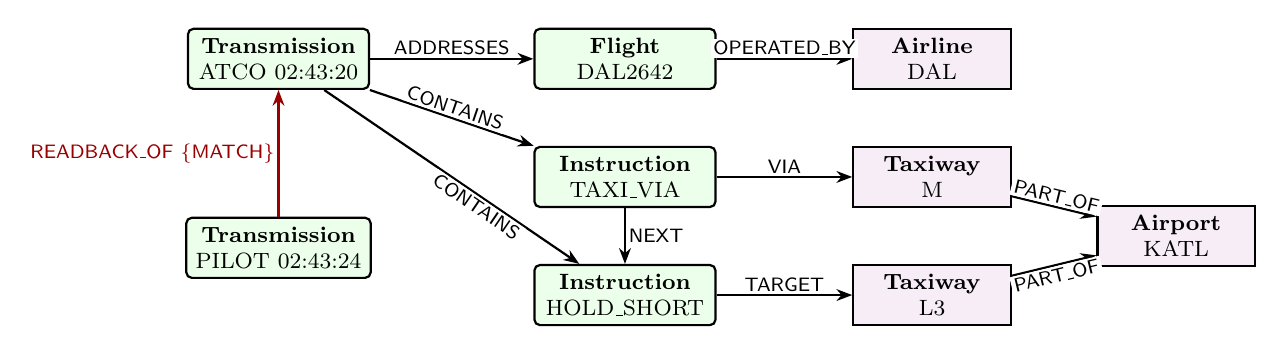
\begin{tikzpicture}[font=\footnotesize,
 dyn/.style={draw,thick,rounded corners=2pt,fill=green!8,minimum height=0.75cm,minimum width=2.3cm,align=center},
 sta/.style={draw,thick,fill=violet!7,minimum height=0.75cm,minimum width=2.0cm,align=center},
 e/.style={-{Stealth[length=2mm]},thick}, l/.style={font=\scriptsize\sffamily,fill=white,inner sep=1pt}]
\node[dyn] (t1) at (0,0) {\textbf{Transmission}\\ATCO 02:43:20};
\node[dyn] (t2) at (0,-2.4) {\textbf{Transmission}\\PILOT 02:43:24};
\node[dyn] (f) at (4.4,0) {\textbf{Flight}\\DAL2642};
\node[sta] (al) at (8.3,0) {\textbf{Airline}\\DAL};
\node[dyn] (i1) at (4.4,-1.5) {\textbf{Instruction}\\TAXI\_VIA};
\node[dyn] (i2) at (4.4,-3.0) {\textbf{Instruction}\\HOLD\_SHORT};
\node[sta] (m) at (8.3,-1.5) {\textbf{Taxiway}\\M};
\node[sta] (l3) at (8.3,-3.0) {\textbf{Taxiway}\\L3};
\node[sta] (ap) at (11.4,-2.25) {\textbf{Airport}\\KATL};
\draw[e] (t1)--node[l,above]{ADDRESSES}(f);
\draw[e] (f)--node[l,above]{OPERATED\_BY}(al);
\draw[e] (t1)--node[l,sloped,above]{CONTAINS}(i1);
\draw[e] (t1)--node[l,sloped,below,pos=0.62]{CONTAINS}(i2);
\draw[e] (i1)--node[l,above]{VIA}(m);
\draw[e] (i2)--node[l,above]{TARGET}(l3);
\draw[e] (m)--node[l,above,sloped]{PART\_OF}(ap);
\draw[e] (l3)--node[l,below,sloped]{PART\_OF}(ap);
\draw[e,red!60!black] (t2)--node[l,left,text=red!60!black]{READBACK\_OF \{MATCH\}}(t1);
\draw[e] (i1)--node[l,right]{NEXT}(i2);
\end{tikzpicture}
\end{center}

%==========================================================
\section{미국·유럽 차이와 우리가 바꾼 것}
%==========================================================
\begin{center}\small
\begin{tabularx}{\textwidth}{@{}>{\raggedright\arraybackslash}p{3.6cm}>{\raggedright\arraybackslash}X>{\raggedright\arraybackslash}X@{}}
\toprule
층위 & 미국·유럽 차이 \cite{chen2023,helmke2025loss} & 이 온톨로지의 처리\\\midrule
어휘 & niner/nine, Juliet/Juliett, Whisky/Whiskey, altimeter(미국)/QNH(유럽) & 정규화 규칙과 STT 프롬프트에 미국 표현 반영\\
표기 & 미국은 쉼표·대문자로 의미를 일부 표시, 유럽은 표기 규칙이 더 엄격 & 개념 단계에서 정규화하므로 영향 없음\\
명령 표현 & 미국 지상관제의 ``monitor tower'', ``give way'' 빈도 & \cmd{MONITOR}를 \cmd{CONTACT}와 분리, \cmd{GIVE\_WAY} 포함\\
세부 정보 & 유럽은 ``continue taxi'', 조건부 허가를 표현. 미국은 일부 생략 & 조건부 허가는 미구현\\
복창 규정 & FAA와 ICAO의 필수 항목이 대부분 겹치지만 완전히 같지 않음 & 지역별 $\mathcal{T}_{\mathrm{req}}^{\rho}$ 매개변수\\
\bottomrule
\end{tabularx}
\end{center}

%==========================================================
\section{한계와 향후 과제}
%==========================================================
\begin{caveat}
\begin{itemize}[leftmargin=12pt]
\item \textbf{공식 파일 미사용:} SESAR와 MITRE 온톨로지는 기계가 읽을 수 있는 공개 파일이 없어 논문 기술만 참고했다. 명령 이름 일부는 대응을 확인하지 못했다(``확인 필요'' 표시).
\item \textbf{조건부 허가 미지원:} ``after the landing traffic, line up and wait'' 같은 조건을 표현하지 못한다.
\item \textbf{설계값:} $T_{\max}$와 대체 규칙은 운영 규정이 아니라 데모용 설계값이다.
\item \textbf{OWL/RDF 미제공:} 현재는 JSON 설정과 코드 검사로 구현했다. atmonto·AIXM IRI를 노드 속성(\texttt{iri})으로만 연결했다.
\item \textbf{향후:} 조건부 허가 추가, SHACL 파일로 제약 분리, 캐나다·유럽 데이터로 ICAO 규정 검증(RQ4), 원저자에게 공식 온톨로지 사양 요청.
\end{itemize}
\end{caveat}

%==========================================================
\begin{thebibliography}{99}\small
\bibitem{helmke2018} Helmke, H., Slotty, M., Poiger, M., Ferrer Herrer, D., Ohneiser, O., Vink, N., Cerna, A. et al. Ontology for Transcription of ATC Speech Commands of SESAR 2020 Solution PJ.16-04. \emph{37th DASC}, 2018. doi:10.1109/DASC.2018.8569238. \url{https://elib.dlr.de/123237}
\bibitem{helmke2021sid} Helmke, H., Shetty, S., Kleinert, M., Ohneiser, O., Ehr, H., Cerna, A. et al. Measuring Speech Recognition and Understanding Performance in Air Traffic Control Domain Beyond Word Error Rates. \emph{SESAR Innovation Days}, 2021. \url{https://publications.idiap.ch/attachments/papers/2021/Helmke_SESARINNOVATIONDAYS_2021.pdf}
\bibitem{kleinert2021} Kleinert, M., Helmke, H., Shetty, S., Ohneiser, O., Ehr, H., Prasad, A., Motlicek, P., Harfmann, J. Automated Interpretation of Air Traffic Control Communication: The Journey from Spoken Words to a Deeper Understanding of the Meaning. \emph{40th DASC}, 2021. doi:10.1109/DASC52595.2021.9594387
\bibitem{helmke2021} Helmke, H. et al. Readback Error Detection by Automatic Speech Recognition to Increase ATM Safety. \emph{14th USA/Europe ATM R\&D Seminar}, 2021.
\bibitem{chen2023} Chen, S., Helmke, H., Tarakan, R.~M., Ohneiser, O., Kopald, H., Kleinert, M. Effects of Language Ontology on Transatlantic Automatic Speech Understanding Research Collaboration in the Air Traffic Management Domain. \emph{Aerospace} 10(6):526, 2023. doi:10.3390/aerospace10060526
\bibitem{helmke2025loss} Helmke, H., Clarke, S.~S., Ohneiser, O., Kleinert, M., Shetty, S., Kalyanam, K. Automatic Speech Recognition and Understanding in Air Traffic Control -- How Much Information Is Lost Over the Atlantic Ocean? \emph{DASC}, 2025. \url{https://ntrs.nasa.gov/citations/20250001345}
\bibitem{faa7110} FAA. \emph{Order JO 7110.65, Air Traffic Control}, §2-4-3 Pilot Acknowledgment/Readback, §3-7-2 Taxi and Ground Movement Operations. (최신판 조항 번호 재확인 필요)
\bibitem{faa7340} FAA. \emph{Order JO 7340.2, Contractions}.
\bibitem{icao4444} ICAO. \emph{Doc 4444, PANS-ATM}. (복창 요건 조항 번호는 최신판에서 확인 필요)
\bibitem{keller2017} Keller, R.~M. \emph{The NASA Air Traffic Management Ontology}. NASA/TM-2017-219526, 2017. \url{https://data.nasa.gov/docs/ontologies/atmonto/index.html}
\bibitem{aixm} EUROCONTROL/FAA. \emph{Aeronautical Information Exchange Model (AIXM) 5.1}; AMD encoding guidance for TaxiHoldingPosition.
\bibitem{naryw3c} Noy, N., Rector, A. (eds.) \emph{Defining N-ary Relations on the Semantic Web}. W3C Working Group Note, 2006.
\bibitem{shacl} Knublauch, H., Kontokostas, D. (eds.) \emph{Shapes Constraint Language (SHACL)}. W3C Recommendation, 2017.
\bibitem{zep2025} Rasmussen, P. et al. Zep: A Temporal Knowledge Graph Architecture for Agent Memory. arXiv:2501.13956, 2025.
\end{thebibliography}
\end{document}
